% Metódy inžinierskej práce

\documentclass[10pt,twoside,slovak,a4paper]{article}

\usepackage[slovak]{babel}
%\usepackage[T1]{fontenc}
\usepackage[IL2]{fontenc} % lepšia sadzba písmena Ľ než v T1
\usepackage[utf8]{inputenc}
\usepackage{graphicx}
\usepackage{url} % príkaz \url na formátovanie URL
\usepackage{hyperref} % odkazy v texte budú aktívne (pri niektorých triedach dokumentov spôsobuje posun textu)

\usepackage{cite}
%\usepackage{times}

\pagestyle{headings}

\title{Gamifikácia pre učenie cudzích jazykov\thanks{Semestrálny projekt v predmete Metódy inžinierskej práce, ak. rok 2022/23, vedenie: Ing. Fedor Lehocki, PhD.}} % meno a priezvisko vyučujúceho na cvičeniach

\author{Branislav Trstenský\\[2pt]
	{\small Slovenská technická univerzita v Bratislave}\\
	{\small Fakulta informatiky a informačných technológií}\\
	{\small \texttt{xtrstenskyb@stuba.sk}}
	}

\date{\small 30. september 2022} % upravte



\begin{document}

\maketitle

\begin{abstract}

Dnešný globálny svet vyžaduje potrebu znalosti jedného alebo viacerých cudzích jazykov. Gamifikácia vo výučbe cudzích jazykov uľahčuje zvládnutie cudzieho jazyka a zároveň  motivuje k udržiavniu a neustálemu zlepšovaniu získaných vedomostí.
Prostredníctvom hry, ktorá je vizuálne zaujímavá, zábavná a ktorá rôznymi odmenami motivuje hráča pokračovať v hre, študent cudzieho jazyka získava vedomosti a zručnosti a má spätnú väzbu o svojom napredovaní.
V súčasnej dobe už existujú niektoré aplikácie určené študentom alebo učiteľom, ktoré využívajú princípy gamifikácie v praxi.

\end{abstract}


\section{Úvod}

Ako napredujú technológie a svet sa stáva prepojenejším, potreba znalosti cudzích jazykov stúpa. Či už ide o zamestnanie v zahraničí, alebo prístup k širšiemu výberu informácií. Učenie cudzích jazykov však vyžaduje časté opakovanie a upevňovanie znalostí, ktoré môže byť ťažké pre študenta dlhodobo udržať. 

Gamifikácia poskytuje zdroj motivácie a pomáha udržiavať pravidelné štúdium. Príkladom gamifikácie je napr. získavanie bodov za skúšky, zábavné minihry alebo notifikácie, ktoré pripomínajú pokračovanie výučby.

Tento článok vysvetlí gamifikáciu všeobecne (časť \ref{gamifikacia}), predstaví spôsoby ako prvky gamifikácie môžu pomôcť pri štúdiu cudzích jazykov (časť \ref{prvky}) a následne uvedie a popíše konkrétne aplikácie, ktoré využívajú princípi gamifikácie v praxy (časť \ref{prax}).

\section{Gamifikácia} \label{gamifikacia}

Okrem zábavných prvkov, hry umožňujú počas hrania rozvíjanie viacerých kognitívnych schopností, ako napríklad logiku, motorické schopnosti, priestorovú orientáciu alebo jazykové schopnosti. 

Vo väčšine prípadov, proces učenia prebieha intuitívne a spontánne počas hrania. Aj keď učenie nie je hlavným cieľom hry, tréning schopností je výsledkom zapájania sa do úloh, ktoré hra vyžaduje, procesu pokus-omyl a ich neustáleho opakovania v rámci hernej slučky. Rozvíjanie schopností je ďalej motivované odmenami, alebo len pocitom prekonania výziev \cite{Rego}.

Gamifikácia je proces, pri ktorom sa prvky hier, považované tradične ako zábavné, používajú priamo na podporu učenia, angažovania a zručností pri riešení problémov. Tieto prvky tvoria systém, v ktorom účastníci prekonávajú výzvy, ktoré obsahujú pravidlá, interaktivitu a spätnú väzbu.

Konkrétne aspekty učenia, ktoré sú vylepšené gamifikáciou sú napriklad spolupráca, participatívny prístup, samoriadené štúdium, motivácia na dokončenie zadaní alebo zjednodušenie hodnotenia \cite{Kapp}.

\section{Prvky gamifikácie} \label{prvky}

Existuje viacero spôsobov ako kategorizovať jednotlivé prvky gamifikácie. Na účely tohto článku sa použije rozdelenie na ciele, mechaniky, estetiku, herné rozmýšľanie, spoluprácu, odmeny, spätnú väzbu a postup cez úrovne.

\begin{figure*}[tbh]
\centering
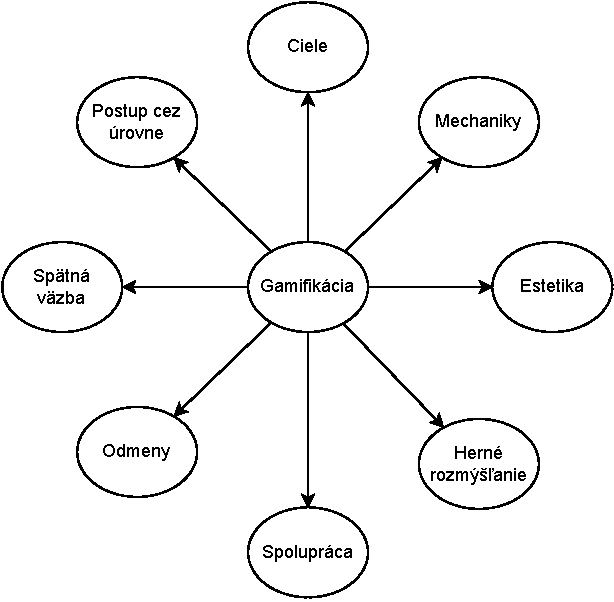
\includegraphics[scale=0.75]{prvky.pdf}
\caption{Prvky gamifikácie}
\label{f:prvky}
\end{figure*}

\subsection{Ciele}

Je dôležité aby sa ciele hry sústredili priamo na učenie, inak vzniká riziko, že študent dokončí hru bez konkrétnych učebných výsledkov. Ďalej je potrebné vytvoriť prechodné ciele, ktoré sa splnia na ceste k hlavným cieľom. Vďaka nim je študent motivovaný, aby pokračoval v hre a je mu poskytnutá spätná väzba o jeho zručnostiach.

\subsection{Mechaniky}

Mechaniký sú tvorené pravidlami, ktoré určujú priebeh hry. Diktujú ako hra funguje, formalizujú štruktúru ktorá podporuje funkcionalitu hry a riadia proces učenia počas hry. V prípade, že má hra sociálne prvky, sú potrebné aj pravidlá na kontrolu kontaktu medzi hráčmi \cite{Rego}.

\subsection{Estetika}

Estetika je dôležitá na udržanie záujmu hráča. Cieľom estetiky je vytvoriť prostredie, ktoré hráča ponorí do hry. Hlavnými faktormi estetiky sú vhodné a vzájomne zrovnané grafické prvky, pozornosť k detailom \cite{Kapp}. a vyvarovanie sa rušivým prvkom. Dôležité je brať do úvahy cieľovú skupinu, pre ktorú je hra určená, ako napríklad ich vekové kategórie. \cite{Rego}

\subsection{Herné rozmýšlanie}

Herné rozmýšľanie je premena tradičných učebných aktivít na herné aktivity. Spočíva v pozorovaní výučbových situácií a identifikovaní prvkov, ktoré je možné obohatiť gamifikáciou. Následne sa vytvoria systémy, ktoré motivujú toto želané správanie \cite{Werbach+Hunter}.

\subsection{Spolupráca}

Aj keď gamifikované zážitky, zamerané na samoštúdium sú dostačujúce, spolupráca môže zlepšiť ich účinnosť. Cez výmenu skúseností a vzájomnú pomoc medzi študentmi sa spoluhráči viac zapájajú do procesu výučby. Skupinová práca tiež vytvára záväzok, ktorý zabraňuje vyhýbaniu sa výučbe \cite{Rego}.

\subsection{Odmeny}

Systémy odmeňovania ako napríklad skóre, hviezdy alebo odznaky sú dôležité pre motiváciu. Aj keď sú odmeny virtuálne, aj tak možnosť niečo vyhrať motivuje hráča pokračovať. Tieto benefity sú zvýšené v sociálnom kontexte, kde jednotlivý študenti môže súperiť medzi sebou. Súperenie je možné využiť prostredníctvom jednoduchých herných prvkov ako zoraďovanie hráčov podľa skóre, kde sa hráč môže sústrediť na zlepšenie svojho miesta. Toto poradie tiež ponúka hráčovi spätnú väzbu. \cite{Kapp}

\subsection{Spätná väzba}

V hrách je spätná väzba, na rozdiel od tradičnej výučby, konštantne k dispozícií. Spätnú väzbu môžeme deliť na informačnú, ktorá ukazuje študentovi stupeň úspešnosti alebo chyby a edukačnú, ktorá mu pomáha k lepšiemu výkonu. Spätná väzba by mala byť prezentovaná tak aby sa o ňu hráč zaujímal. Hodnotenie by malo byť tiež opakovateľné, aby ho mal hráč možnosť zlepšiť.  \cite{Kapp}

\subsection{Postup cez úrovne}

Postup cez úrovne má tri úlohy:
\begin{enumerate}
	\item Zmenu častí priebehu hry, aby bola udržaná pozornosť hráča
	\item Zvýšenie náročností úloh, na pokračovanie vývinu zručností
	\item Tvorba motivácie cez pocit prekonania výzvy
\end{enumerate}
Prostredníctvom úrovní si hry môžu udržať konzistentnú obtiažnosť vzhľadom na zlepšené zručnosti hráča a predísť tomu aby sa hra stala príliš jednotvárna a únavná. \cite{Kapp}

\section{Gamifikácia výučby jazyka v praxi} \label{prax}

Už existuje veľký počet nástrojov, ktoré využívajú gamifikáciu pre výučbu jazyka.

\begin{table*}[tbh]
\centering
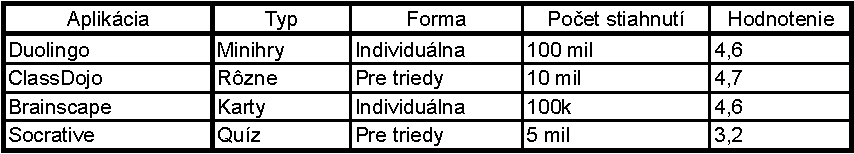
\includegraphics[scale=1.0]{aplikacie.pdf}
\caption{Aplikácie využívajúce gamifikáciu.}
\label{f:aplikacie}
\end{table*}


\subsection{Duolingo}

Duolingo je mobilná aplikácia dostupná pre IPhone aj Android, kde používatelia postupujú a učia sa cez úrovne. Táto aplikácia má viac ako 300 miliónov používateľov \cite{Frederic}. Duolingo ponúka výučbu veľkého počtu jazykov. Počet možností je obmedzený jazykom, v ktorom sú lekcie vytvorené. Pre študentov so znalosťou češtiny je k dispozícii iba anglický kurz, ale ľudia so znalosťou angličtiny sa môžu učiť 40 rôznych jazykov \cite{Duolingo}.

Táto aplikácia efektívne pokrýva oblasti reči, gramatiky, počúvania a slovnej zásoby. Kurzy sa prispôsobujú individuálnemu štýlu učenia sa používateľa. Lekcie sú rozdelené do tém, ktoré obsahujú úlohy. Po zvládnutí úloh je študent odmenený virtuálnou menou. Aplikácia tiež odmeňuje rôzne úspechy odznakmi, napríklad ak používateľ prejde celú lekciu bez chyby. Duolingo je určená hlavne pre samoštúdium, ale má aj funkcie, ktoré umožňujú kontrolu postupu učiteľmi \cite{Prathyusha}.

\subsection{ClassDojo}

ClassDojo je k dispozícií ako mobilná aplikácia pre IPhone aj Android, aj ako webová stránka. Aplikácia pracuje ako komunikačná platforma, kde študenti môžu zdieľať svoje výsledky. Učitelia udeľujú študentom body, za ktoré sú študenti zoradení do rebríčku. Spätná väzba je tak k dispozícií ihneď po odovzdaní úloh. ClassDojo umožňuje tiež toto hodnotenie zdieľať z rodičmi \cite{Prathyusha}.

Aplikácia sa používa v 95\% základných škôl v USA aj v ďalších 180 krajinách. \cite{Chaykowski}

\subsection{Brainscape}
Brainscape dostupná ako mobilná aplikácia aj cez webový prehliadač. Používateľovi ponúka rýchlo tempový kvíz prostredníctvom kariet. Výsledky sú aplikáciou následne analyzované, čo umožňuje optimalizáciu výučby tak, že zdôrazňuje prvky, ktoré sú pre užívateľa náročné. Tento iteratívny proces pomáha pri prehlbovaní porozumenia učiva a uchovaniu informácií \cite{Brainscape}.

V kontexte výučby jazyka Brainscape ponúka výučbu slovnej zásoby a konštrukcie viet. Pre niektoré jazykové karty sú k dispozícií aj audio nahrávky \cite{Prathyusha}.

\subsection{Socrative}
Socrative je mobilná aplikácia dostupná pre IPhone aj Android, ale aj cez webový prehliadač. Je určená pre učiteľov, ktorí môžu tvoriť kvízy pre studentov. Aplikácia študentovi poskytuje okamžitú spätnú väzbu a zhromažďuje výsledky pre vyučujúceho. 
Tieto aktivity môžu byť voliteľne prezentované ako takzvaný “závod”, kde študenti súperia medzi sebou \cite{Socrative}.


\section{Záver} \label{zaver} % prípadne iný variant názvu
Dnešný globálny svet vyžaduje potrebu znalosti jedného alebo viacerých cudzích jazykov. Gamifikácia vo výučbe cudzích jazykov uľahčuje zvládnutie cudzieho jazyka a zároveň  motivuje k udržiavaniu a neustálemu zlepšovaniu získaných vedomostí.

Z využitím viacerých prvkov gamifikácie, t.j. ciele, mechaniky, estetiku, herné rozmýšľanie, spoluprácu, odmeny, spätnú väzbu a postup cez úrovne, je možné vytvoriť systém, ktorý pomôže pri ich výučbe.

Už existujú aplikácie, ktoré využívajú tieto prvky v praxi, ako napríklad Duolingo, ClassDojo, Socrative a Brainscape. Z ich úspechov je možné usúdiť, že gamifikácia je naozaj účinným nástrojom na učenie cudzieho jazyka.


\section*{Vyjadrenie sa k témam prednášky}

\paragraph{Technológia a ľudia}
Technológia je dôležitou súčasťou moderného života. Ľudia používajú počítače na čítanie správ, hranie hier, štúdium alebo nakupovanie. Ale techológia sa používa aj na komunikáciu medzi ľuďmi t.j. posielanie správ, telefonovanie, chatovanie atď. Týmto sa techológia stáva súčasťou aj procesu socializácie. Technológie nás obklopujú, informujú a zabávajú čim kontrolujú naše životy.

\paragraph{História informatiky}
Históriu informatiky siaha až do pradávnych čias, keď ľudia používali hlinené dosky na uchovanie informácií. Technológia napredovala. Najprv to bol vynález papiera, ktorý vydláždil cestu ku prvej kultúrnej revolúcií - tlačiarenskemu stroju. Týmto sa stali informácie prístupnými pre veľké množstvo ľudí. Ďalšia významná historická udalosť je vynález internetu, čím sa začala informačná doba.

\paragraph{Spoločenské súvislosti informatiky}
Historicky bolo pre ľudí ťažké získať aktuálne informácie o dianí vo svete. To sa však zmenilo s vynálezom internetu. Dnes je obrovské množstvo informácií neustále prístupné. Toto sa stalo veľkým prínosom pre spoločnosť. Ale problémom je, že rovnako, ako sa šíria pravdivé informácie, šíria sa aj tie nepravdivé. Niekedy je veľký problém rozoznať čo je pravda a čo nie. Dezinformácie môžu spôsobiť veľké problémy, keď na nich ľudia zakladajú svoje postoje a rozhodnutia. 

%\acknowledgement{Ak niekomu chcete poďakovať\ldots}

\Urlmuskip=0mu plus 1mu
\def\UrlBreaks{\do\/\do-}

% týmto sa generuje zoznam literatúry z obsahu súboru literatura.bib podľa toho, na čo sa v článku odkazujete
\bibliography{literatura}
\bibliographystyle{plain} % prípadne alpha, abbrv alebo hociktorý iný
\end{document}
